\chapter{Program description}
The program is an IoT system where vehicles can communicate with a server. The server performs calculations to decide the behavior of the vehicles. The program's primary goal is to increase traffic flow and prevent traffic congestion. The system developed in this project has focused on incoming traffic at an intersection. \figref{fig:diagramserver} shows a flow diagram that describes the server in our demonstration, mentioned in \secref{sec:demo}.

Our solution adheres to the requirements Accenture set for us. As per discussed in \secref{sec:goals} the vehicles can also drive independently. Moreover, the server can establish multiple connections and determine the optimal speed of each vehicle depending on the incoming situation at an intersection. During the demonstration shown in \secref{sec:demo}, it became apparent that the outcome differs; when the cars were driving solely on the integrated AI in contrast to being connected to the server.
\begin{figure}[h!]
	\centering
	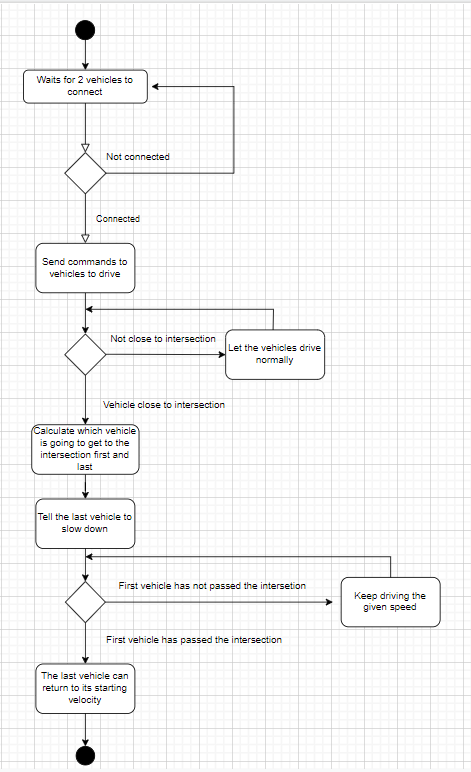
\includegraphics[width=1\linewidth]{figures/Flow_diagram_server}
	\caption[Flow diagram server]{Flow diagram for the server. This diagram specificly shows the flow of the semi physical demonstration.}
	\label{fig:diagramserver}
\end{figure}
\clearpage
%\section{Preface}

The product documentation is a technical description of the product.

The product documentation assumes the reader has some prior knowledge in basic programming.
%\section{Program description}

\begin{figure}[h!]
	\centering
	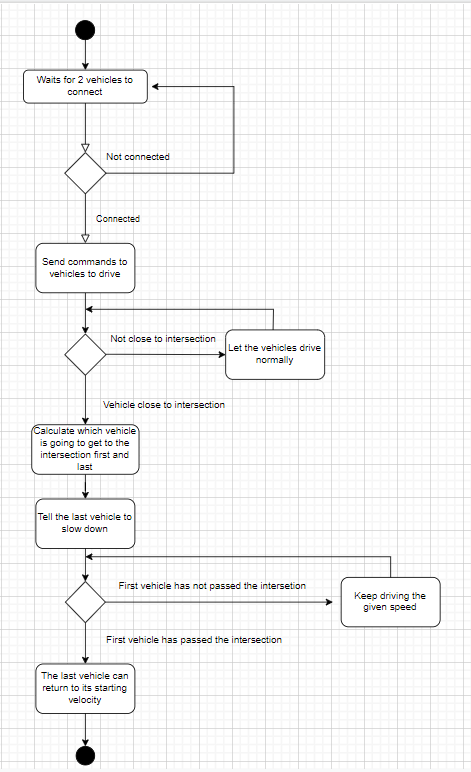
\includegraphics[width=1\linewidth]{figures/Flow_diagram_server}
	\caption[Flow diagram server]{Flow diagram for the server. This diagram specificly shows the flow of the semi physical demonstration.}
	\label{fig:diagramserver}
\end{figure}

The program is an IoT-system were vehicles can communicate with eachother through a server. It constists of a server which has the responsibility for the calculations and decision making, and a client which are the vehicles. The function of the program is to increase traffic flow and prevent traffic congestion. As of now the program can be used in an intersection with two vehicles, but can be scaled to include more vehicles. Here is a diagram that describes the flow of our server in the demonstration:




%\section{Adherence to project requirements}
Our solution adheres to the requirements Accenture set for us. Our prototype cars can work both with, and without being connected to a server. The server can handle multiple connections and adjust trafic based on the situation on the road. Through er deomnstration we also showed a situation where the outcome differs depending on if the cars are connected to the server or just driving on the on-board AI.


%\section{Server flow diagram}
% \chapter{User manual}\label{sec:user_manual}
We have written a manual for people who want to recreate our demonstration. The demonstration could for example be shown off at exhibitions. The manual could also be used for people who want to further test and develop our IoT-system.

First check the IP-address of the internet you are connected to, and the usable ports. Make sure that your computer hosting the server and the vehicles are connected to the same network.

\begin{lstlisting}
$ipconfig getifaddr en0
192.168.56.208
\end{lstlisting}

Then open the Server solution in your code editor, we have used visual studio. Under the folder “properties” there is a file called launchSettings.json. In that file write in the ip address and the port in the applicationUrl-section:

\begin{json}
"profiles": {
	"SignalRServer": {
		"commandName": "Project",
		"dotnetRunMessages": true,
		"launchBrowser": false,
		"applicationUrl": "https://192.168.56.208:7058;http://192.168.56.208:5048",
		"environmentVariables": {
			"ASPNETCORE_ENVIRONMENT": "Development"
		}
	},
\end{json}
	
After that, open the Client solution. Here we used Pycharm as the IDE. Open the config.json document and replace the same IP address and port:
	
\begin{json}
"client": {
	"host": "192.168.56.208",
	"port": 5048,
	"delay": 0.1
},
\end{json}
	
	If the vehicles have not connected to that network before, they need to log on to that network. To log on to a new network; connect the Raspberry Pi to a power source and a display, and use the user interface. The display port on the Raspberry Pi is a micro USB port. When the Raspberry Pi has booted up, click on the internet icon and connect to the same network as the server. If the network has been connected to it before, Raspberry Pi will automatically connect to that network during boot up.
	
	The initial speed of the vehicles can be changed by adjusting the value of \verb|SpeedLimit| located at VehicleHubDatabase under the Database folder on the server solution:
\begin{csharp}
public class VehiclesHubDatabase : IVehiclesHubDatabase
{
	...
	public double SpeedLimit => 80;
	...
}
\end{csharp}
Moreover, the configuration of the road can also be changed by changing the following section of the code:
\begin{csharp}
public class VehiclesHubDatabase : IVehiclesHubDatabase
{
	...
	public VehiclesHubDatabase()
	{
		_intersection = new Intersection().
			AddRoad(new Road {Length = 300}.
				AddLane(null, true).
				AddLane()).
			AddRoad(new Road {Length = 300}.
				AddLane(null, true).
				AddLane());
		...
	}
	...
}
\end{csharp}
The current configuration shown above corresponds to the same configuration shown in \figref{fig:intersectionconcept}. The intersection can be moved by adding additional arguments such as:
\begin{csharp}
	public class VehiclesHubDatabase : IVehiclesHubDatabase
	{
		...
		public VehiclesHubDatabase()
		{
			_intersection = new Intersection().
				AddRoad(new Road {Length = 300}.
					AddLane(null, true).
					AddLane(), 200).
				AddRoad(new Road {Length = 300}.
					AddLane(null, true).
					AddLane(), 150);
			...
		}
		...
	}
\end{csharp}
\figref{fig:altintersectionconfig} shows the resulting topology by adding extra parameters to the code above.
\begin{figure}[h!]
	\centering
	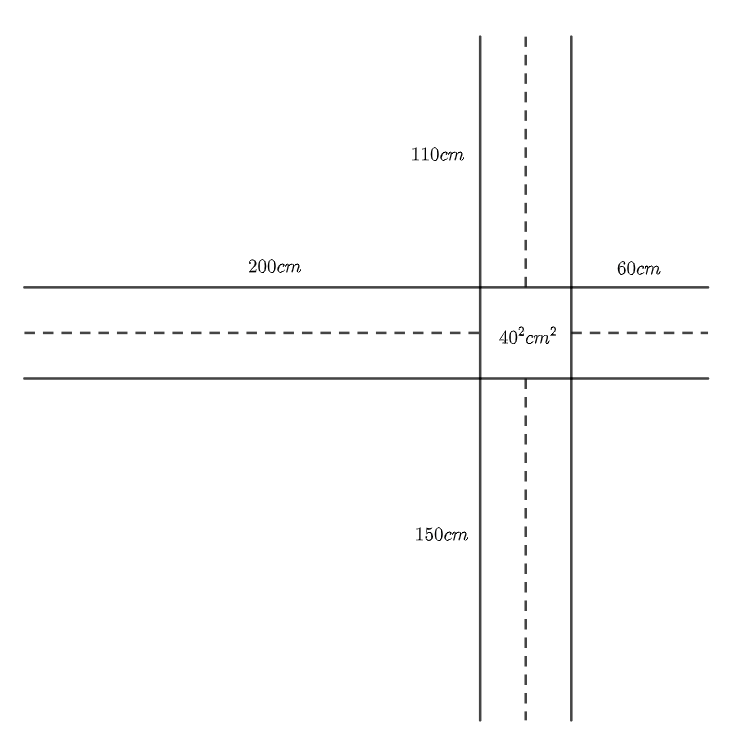
\includegraphics[width=1\linewidth]{figures/alt_intersection_config}
	\caption{An alternative configuration of the intersection and its connected roads by adding extra parameter to the initialization of the intersection as described by the previous code snippet.}
	\label{fig:altintersectionconfig}
\end{figure}

The length is in centimeters and needs to correlate with the length of the physical track. We used tape to show where the roads were. However, this is unnecessary. We recommend a track between three to four meters long for the best results.

Lastly, position both vehicles down at the start of the two tracks, turn on the server and connect to the power banks. The vehicles should automatically connect to the server after 20-30 seconds. When both vehicles have established a connection to the server, the demonstration has started.
\section{Product specification}
The main part of this project is to develop a client-server communication system, with the purpose of producing a physical simulation on how a centralized system can contribute to an improved traffic flow. Due to the nature of this project, no graphical user interfaces has been developed. Hence, it is deemed necessary to present key parts of the code that are responsible for such a system to work. This section will therefore elaborate, in detail, how essential code snippets are interacting with each to produce the result.

Furthermore, the code that has been written during this project has been written in the languages Python and C\# using Pycharm and Rider IDE respectively. Therefore, syntax highlighting has also been used to best simulate the same syntax highlighting used in both IDE respectively. In addition, some artistic freedom has been used to present the code snippets; the symbol \verb|...| has been used to indicate irrelevant code to the current discussion and the symbol  \textcolor{red}{$\hookrightarrow$} simply means that the line of code following \textcolor{red}{$\hookrightarrow$} is on the same line above but is broken up due to lack of space. Also, each code snippets starts with the class and method it belongs to.
\subsection{Initialization}\label{initialization}
\subsubsection{Client.py}
The client package is an essential module in the Raspberry Pi vehicles for the success of this project. The client class is mainly responsible for connecting, handling, and sending data to the server. The client class does not aim to be used alone but rather as a superclass for other IoT devices. Hence, it should be inherited and handle everything that pertains to client-server communication in the background.

The client's init method does several things: It reads from the config.json file to store the defined host and port it will use to establish a connection to the server.
\begin{python}
class Client:
	def __init__(self, properties=None, **kwargs):
		...
		with open("client/config.json") as f:
			config = json.load(f).get('client')
			if config is not None:
				self.__uri = f"://{config.get('host')}:{config.get('port')}/{self.__class__.__name__.lower()}sHub"
				self.__delay = config.get('delay')
		...
\end{python}

Then, it starts a negotiation process with the server, where it receives a connection id that the client will use during its connection lifetime to the hub.

\begin{python}
class Client:
	def __init__(self, properties=None, **kwargs):
		...
		urllib3.disable_warnings()
		response = requests.post(f"http{self.__uri}/negotiate?negotiateVersion=0", verify=False)
		self.connection_id = response.json().get("connectionId")
		self.websocket_uri = f"ws{self.__uri}?id={self.connection_id}"
		...
\end{python}

The client also gives itself a random id stored as one of its properties. The client's id is also stored on the server and is mainly used to retrieve and update the client's information.

Furthermore, \verb|Client.__init__| also stores a dictionary of events.
\begin{python}
class Client:
	def __init__(self, properties=None, **kwargs):
		...
		self.subscribed_events = {
			"disconnect": self.disconnect,
			"force_patch": self.force_patch,
			"continuously_patch": self.continuously_force_patch
		}
		...
\end{python}

Values in this dictionary are references to functions in this class and is used to invoke certain behaviours by the server. For instance, \newline\verb|await Clients.Client(Context.ConnectionId).SendAsync("disconnect");| from the server will call \verb|def disconnect(self)| in the client. 

\subsubsection{Vehicle.py}
The vehicle class contains all the data and methods of the vehicle. Furthermore, \verb|class Vehicle(Client)| inherits the client class which enables \verb|Vehicle| to perform all the necessary operations to establish connection upon initiation. An important remark is that \verb|Client| performs the negotiation to the server using endpoint \newline \verb|{self.__class__.__name__.lower()}sHub/negotiate?negotiateVersion=0| meaning that through inheritence and initialization of \verb|Vehicle|, the subclass negotiates with the endpoint  \verb|vehiclesHub/negotiate?negotiateVersion=0|, which is mapped in \verb|Program.cs| with
\begin{csharp}
...
app.MapHub<VehiclesHub>("/vehiclesHub");
...
\end{csharp}

Furthermore, \verb|Vehicle| also reads from \verb|config.json| to define it's initial properties with the snippet shown below:
\begin{python}
class Vehicle(Client):
	def __init__(self, properties=None, **kwargs):
		...
		if properties is None and len(kwargs) == 0:
			with open("client/config.json") as f:
				config = json.load(f).get('vehicle')
				if config is not None:
					self.properties.update(config)
		...
\end{python}

\verb|Vehicle| also utilizes the property builder of \verb|Client|.

\begin{python}
class Vehicle(Client):
	def __init__(self, properties=None, **kwargs):
		...
		self.property_builder(
			required={'length', 'height', 'width', 'mass'},
			optional={'velocity': 0, 'position': 0, 'travel_plan': None},
		)
		...
\end{python}

In short, the property builder is used to define the required properties of the vehicle class. The meaning is to restrict somewhat what data the vehicle class should contain. If one should directly initialize Vehicle without using config.json, one must assign values to length, height, width, and mass.

Lastly, \verb|Vehicle| adds subscribed events that the server can invoke:
\begin{python}
class Vehicle(Client):
	def __init__(self, properties=None, **kwargs):
		...
		self.subscribed_events.update({
			"adjust_velocity": self.adjust_velocity
		})
\end{python}

Likewise, as in \verb|Client|, should other events be required for a vehicle, one can add it to the dictionary as proposed above.
\subsection{Handshake and listener}\label{handshake}
After initializing the vehicle class as a client with
\begin{python}
async def main():
	...
	client = Vehicle()
	...
\end{python}
then the client's \verb|listen| method can be called:
\begin{python}
async def main():
	...
	listener = asyncio.create_task(client.listen())
	...
\end{python}
The listener method is responsible for handling responses and requests from the server. Hence, it must run concurrently as the vehicle continuously sends data to the server.

When the listener is called, the client performs the following code:
\begin{python}
class Client:
...
	async def listen(self):
	async with websockets.connect(self.websocket_uri) as websocket:
		self.__websocket = websocket
		await self.__handshake()
		await self.__listen()
...
\end{python}
The method first opens a WebSocket connection using the stored URI and stores this as a private variable. Then, a handshake with the server is performed:
\begin{python}
class Client:
...
	async def __handshake(self, protocol: str = "json", version: int = 1):
		data = self.signalr_encode_message({"protocol": protocol, "version": version})
		await self.__websocket.send(data)
		response = self.signalr_decode_message(await self.__websocket.recv())
		if "error" in response:
			print(response)
		else:
			await self.send_non_blocking("AddClient", self.properties)
...
\end{python}

The code above describes the handshake process between the client and the server. First, the client informs the server of the protocols it will use throughout its lifetime. Then, it stores the client, in this case, the vehicle, to the server using the defined properties.

Further elaboration, the client invokes the method
\begin{csharp}
public partial class VehiclesHub : Hub
{
	...
	public async Task AddClient(JsonDocument jsonDocument) {...}
	...
}
\end{csharp}
on the server. This method first creates a vehicle with all the provided information sent by the client
\begin{csharp}
public partial class VehiclesHub : Hub
{
	...
	public async Task AddClient(JsonDocument jsonDocument)
	{
		...
		var vehicle = Vehicle.Create(jsonDocument);
		...
	}
	...
}
\end{csharp}
using the static method defined by the Vehicle model. In addition, it assigns the travel plan to the vehicle by using values defined by config.json from the client:
\begin{json}
{
	...
	"vehicle": {
		...
		"travel_plan": {
			"start": {
				"road": 0,
				"lane_reversed": false
			},
			"end": {
				"road": 0,
				"lane_reversed": false
			}
		}
	}
}
\end{json}

Furthermore, the vehicle's current lane is also assigned to track which lane the vehicle is driving on. Then, \verb|public class VehiclesHubDatabase| adds the \verb|Vehicle|, together with its connection id \verb|Context.ConnectionId| for easy retrieval.

Moreover, for the sake of the demo, the server is also instructed to wait for a second vehicle to connect before allowing the vehicles to drive
\begin{csharp}
public partial class VehiclesHub : Hub
{
	...
	public async Task AddClient(JsonDocument jsonDocument)
	{
		...
		vehicle.Velocity = 0;
		_database.Update(vehicle);
		await Clients.Client(Context.ConnectionId).SendAsync("adjust_velocity", vehicle);
		await WaitForVehicles(vehicle, _database.SpeedLimit, 2);
	}
	...
}
\end{csharp}
by first setting the vehicle's velocity to zero, updating the new velocity in the database, and adjusting the velocity of the client to zero. Lastly, it calls the \verb|WaitForVehicles| method, which will adjust every client's velocity to the defined \verb|SpeedLimit| in \verb|VehiclesHubDatabase|.

\subsection{Patch}
After initialization and handshake elaborated in \hyperref[initialization]{\ref{initialization} Initialization} and \hyperref[handshake]{\ref{handshake} Handshake and listener} respectively, the Raspberry Pi vehicles starts to drive into an intersection simultaneously. Throughout the journey the cars are continuously patching to the server, by calling the client's \verb|async def send\_patch| method.

\begin{python}
class Client:
	...
	async def send_patch(self, **kwargs) -> None:
		if self.properties_has_changed(**kwargs) or self.__continuously_patch:
			await self.send_invocation("patch", self.properties)
		else:
			await asyncio.sleep(self.__delay)
\end{python}

As seen above \pythoninline{send\_patch} calls the \pythoninline{async def send_invocation} method, which communicates the vehicle's current information by invoking \newline
\verb|public async Task Patch| on \verb|VehiclesHub|.

The patch method on \verb|VehiclesHub| is responsible for handling the behaviour, specifically adjusting the velocity of individual vehicles:
\begin{csharp}
public partial class VehiclesHub : Hub
{
	...
	public async Task Patch(JsonDocument jsonDocument)
	{
		var vehicle = Vehicle.Create(jsonDocument);
		_database.Update(vehicle);
		vehicle = _database.Fetch(vehicle);
		...
	}
}
\end{csharp}
The snippet above shows that the method first creates a new vehicle using the information provided by the \verb|Client|. However, since this new vehicle does not contain all the information, such as the travel plan, the method first update the existing vehicle in the database in order to refresh the vehicle with the available information. It then fetch the same vehicle that was stored in the handshake, mentioned in \hyperref[handshake]{\ref{handshake} Handshake and listener}. Assuming that the vehicle has been successfully retrieved it will then handle this vehicle accordingly:
\begin{csharp}
public partial class VehiclesHub : Hub
{
	...
	public async Task Patch(JsonDocument jsonDocument)
	{
		...
		await HandleIntersection(vehicle);
		await HandleInsideIntersection(vehicle);
		await HandleEndOfRoute(vehicle);
		...
	}
}
\end{csharp}
Shortly summarized \verb|HandleIntersection| is responsible to adjust the velocity of every vehicle approaching the intersection to avoid collisions. Furthermore, \verb|HandleInsideIntersection| increases the speed to \verb|VehiclesHubDatabase| defined \verb|SpeedLimit|. Lastly, \verb|HandleEndOfRoute| ensure that any vehicles that has completed their journey, defined during the handshake, terminates their connection with the server.
\subsection{VehiclesHubDatabase}
The \verb|VehiclesHubDatabase| played a key role in this project. Coming to the realization on \hyperref[phase3]{\ref{phase3} Phase 3 - Signal R} the project needed a database that could handle the continuous changes in each \verb|Vehicle| position in real time. During research the group was unable to conclude on any databases that would fit our requirement. Hence, \verb|VehiclesHubDatanbase| was created to serve as a live in-memory database that could continuously update the positions of each vehicle on each lane.
\begin{figure}[h!]
	\centering
	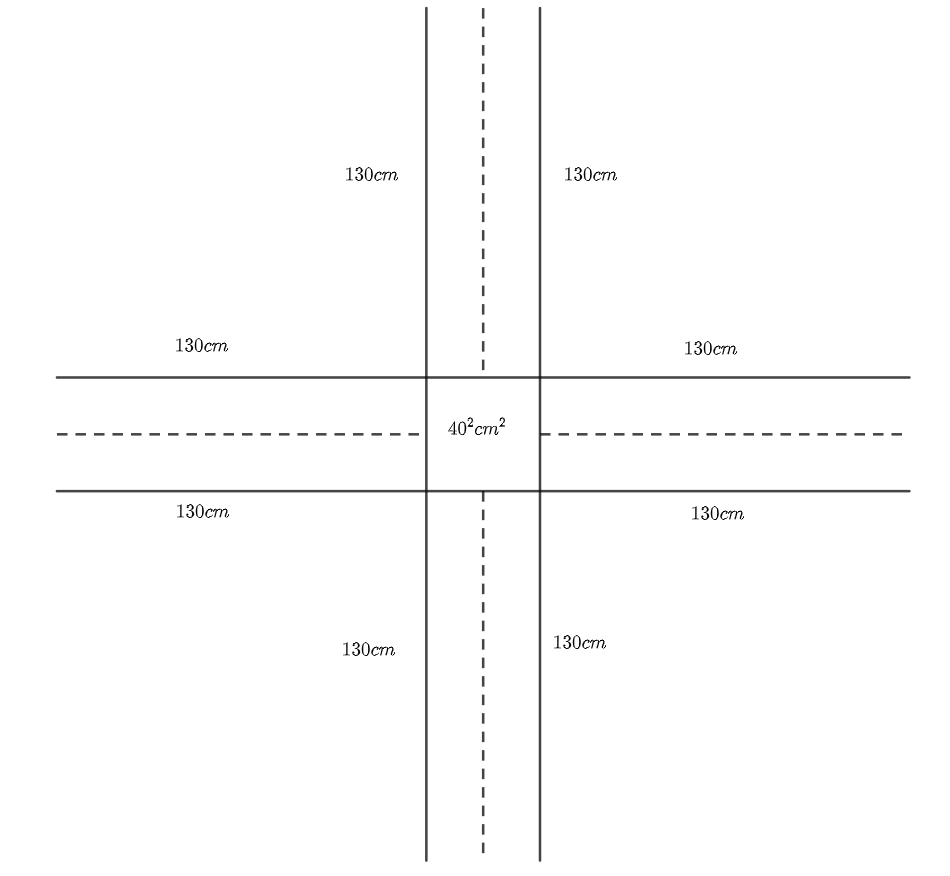
\includegraphics[width=1\linewidth]{figures/intersection_concept}
	\caption{This figure shows two roads each with two lanes and a total length of 300cm. The overlapping part forms a square which is the intersection. This configuration was heavily considered when creating representational models on the server, and also used for the demo as a result.}
	\label{fig:intersectionconcept}
\end{figure}

Before starting with \verb|VehiclesHubDatabase|, it was required to define what a road, lane and intersection is, respectively. Thus, \verb|Road.cs|, \verb|Lane.cs| and \verb|Intersection.cs| was developed. Consequently, \verb|VehiclesHubDatabase| was created.
\begin{csharp}
public class VehiclesHubDatabase : IVehiclesHubDatabase
{
	private readonly Intersection _intersection;
	
	private readonly HashSet<Vehicle> _vehicles = new();
	private readonly HashSet<Lane> _lanes = new();
	public int Count => _vehicles.Count;
	private readonly Dictionary<string, Vehicle> _connectionIds = new();
	private readonly Dictionary<Vehicle, string> _vehiclesConnectionId = new();
	...
	public double SpeedLimit => 80;
	...
}
\end{csharp}

Currently, \verb|VehiclesHubDatabase| only holds one intersection, due to time constraint this was not extended for a configuration with multiple intersections. Moreover, both vehicles and lanes are stored inside a hashset for fast retrieval. In addition, \verb|Count| is used in \verb|WaitForVehicles|, elaborated in sub-section \hyperref[handshake]{\ref{handshake} Handshake and listener}, and \verb|_connectionId| and \verb|_vehiclesConnectionId| is used during \verb|Patch| to invoke \verb|adjust_velocity| on individual vehicles. While, \verb|SpeedLimit| defines the upper speed vehicles are limited to on the two roads shown in \hyperref[fig:intersectionconcept]{Figure \ref{fig:intersectionconcept}}.

The road configuration found in \hyperref[fig:intersectionconcept]{Figure \ref{fig:intersectionconcept}} is defined in the constructor using a builder pattern.
\begin{csharp}
public class VehiclesHubDatabase : IVehiclesHubDatabase
{
	...
	public VehiclesHubDatabase()
	{
		_intersection = new Intersection().
			AddRoad(new Road {Length = 300}.
				AddLane(null, true).
				AddLane()).
		AddRoad(new Road {Length = 300}.
				AddLane(null, true).
				AddLane());
		
		_intersection.ConnectedLanes().
			ForEach(lane => _lanes.Add(lane));
	}
	...
}
\end{csharp}

Lastly, \verb|VehiclesHubDatabase| is added as a singleton service in \verb|Program.cs| to ensure that we have a static database throughout the lifetime of the program:
\begin{csharp}
...
builder.Services.AddSingleton<IVehiclesHubDatabase>(new VehiclesHubDatabase());
...
\end{csharp}

It is also worth to mention some of the core  functionalities of \verb|VehiclesHubDatabase|:

\subsubsection{Adding vehicles}
Calling the \verb|Add| method makes it possible to add vehicles:
\begin{csharp}
public class VehiclesHubDatabase : IVehiclesHubDatabase
{
	...
	public void Add(Vehicle vehicle, string? connectionId = null) {...}
	
	public void Add(Vehicle vehicle, Lane? lane = null) {...}
	...
}
\end{csharp}

\subsubsection{Removing vehicles}
Removing vehicles can be achieved by calling the \verb|Remove| method:
\begin{csharp}
public class VehiclesHubDatabase : IVehiclesHubDatabase
{
	...
	public void Remove(Vehicle vehicle) {...}
	...
}
\end{csharp}

\subsubsection{Updating vehicles}
Updating either a specific information of a vehicle or all vehicles can be done by calling the \verb|Update| method:
\begin{csharp}
public class VehiclesHubDatabase : IVehiclesHubDatabase
{
	...
	public void Update(Vehicle? vehicle = null) {...}
	...
}
\end{csharp}

\subsubsection{Fetching vehicles}
One can fetch an existing vehicle from the database by passing a vehicle with the same GUID with:
\begin{csharp}
public class VehiclesHubDatabase : IVehiclesHubDatabase
{
	...
	public Vehicle? Fetch(Vehicle vehicle) {...}
	...
}
\end{csharp}

\subsubsection{Get the connection Id of a particular vehicle}
By passing a vehicle into
\begin{csharp}
public class VehiclesHubDatabase : IVehiclesHubDatabase
{
	...
	public string? ConnectionId(Vehicle vehicle) {...}
	...
}
\end{csharp}
one can retrieve the connection Id that the given vehicle is using.

\subsubsection{Find vehicles approaching the intersection}
Maybe the most important feature of \verb|VehiclesHubDatabase| is the two method shown below:
\begin{csharp}
public class VehiclesHubDatabase : IVehiclesHubDatabase
{
	...
	public IEnumerable<Vehicle> NextVehiclesIn() {...}
	public IEnumerable<Vehicle> OnlyFirstIntoNextVehiclesIn() {...}
}
\end{csharp}
The first method \verb|NextVehiclesIn| returns a list of vehicles currently approaching the intersection defined in the constructor, ordered with respect to the vehicle closest to the intersection. The latter method \verb|OnlyFirstIntoNextVehiclesIn| returns an ordered list of the closest vehicle per lane.

%\chapter{User manual}\label{sec:user_manual}
We have written a manual for people who want to recreate our demonstration. The demonstration could for example be shown off at exhibitions. The manual could also be used for people who want to further test and develop our IoT-system.

First check the IP-address of the internet you are connected to, and the usable ports. Make sure that your computer hosting the server and the vehicles are connected to the same network.

\begin{lstlisting}
$ipconfig getifaddr en0
192.168.56.208
\end{lstlisting}

Then open the Server solution in your code editor, we have used visual studio. Under the folder “properties” there is a file called launchSettings.json. In that file write in the ip address and the port in the applicationUrl-section:

\begin{json}
"profiles": {
	"SignalRServer": {
		"commandName": "Project",
		"dotnetRunMessages": true,
		"launchBrowser": false,
		"applicationUrl": "https://192.168.56.208:7058;http://192.168.56.208:5048",
		"environmentVariables": {
			"ASPNETCORE_ENVIRONMENT": "Development"
		}
	},
\end{json}
	
After that, open the Client solution. Here we used Pycharm as the IDE. Open the config.json document and replace the same IP address and port:
	
\begin{json}
"client": {
	"host": "192.168.56.208",
	"port": 5048,
	"delay": 0.1
},
\end{json}
	
	If the vehicles have not connected to that network before, they need to log on to that network. To log on to a new network; connect the Raspberry Pi to a power source and a display, and use the user interface. The display port on the Raspberry Pi is a micro USB port. When the Raspberry Pi has booted up, click on the internet icon and connect to the same network as the server. If the network has been connected to it before, Raspberry Pi will automatically connect to that network during boot up.
	
	The initial speed of the vehicles can be changed by adjusting the value of \verb|SpeedLimit| located at VehicleHubDatabase under the Database folder on the server solution:
\begin{csharp}
public class VehiclesHubDatabase : IVehiclesHubDatabase
{
	...
	public double SpeedLimit => 80;
	...
}
\end{csharp}
Moreover, the configuration of the road can also be changed by changing the following section of the code:
\begin{csharp}
public class VehiclesHubDatabase : IVehiclesHubDatabase
{
	...
	public VehiclesHubDatabase()
	{
		_intersection = new Intersection().
			AddRoad(new Road {Length = 300}.
				AddLane(null, true).
				AddLane()).
			AddRoad(new Road {Length = 300}.
				AddLane(null, true).
				AddLane());
		...
	}
	...
}
\end{csharp}
The current configuration shown above corresponds to the same configuration shown in \figref{fig:intersectionconcept}. The intersection can be moved by adding additional arguments such as:
\begin{csharp}
	public class VehiclesHubDatabase : IVehiclesHubDatabase
	{
		...
		public VehiclesHubDatabase()
		{
			_intersection = new Intersection().
				AddRoad(new Road {Length = 300}.
					AddLane(null, true).
					AddLane(), 200).
				AddRoad(new Road {Length = 300}.
					AddLane(null, true).
					AddLane(), 150);
			...
		}
		...
	}
\end{csharp}
\figref{fig:altintersectionconfig} shows the resulting topology by adding extra parameters to the code above.
\begin{figure}[h!]
	\centering
	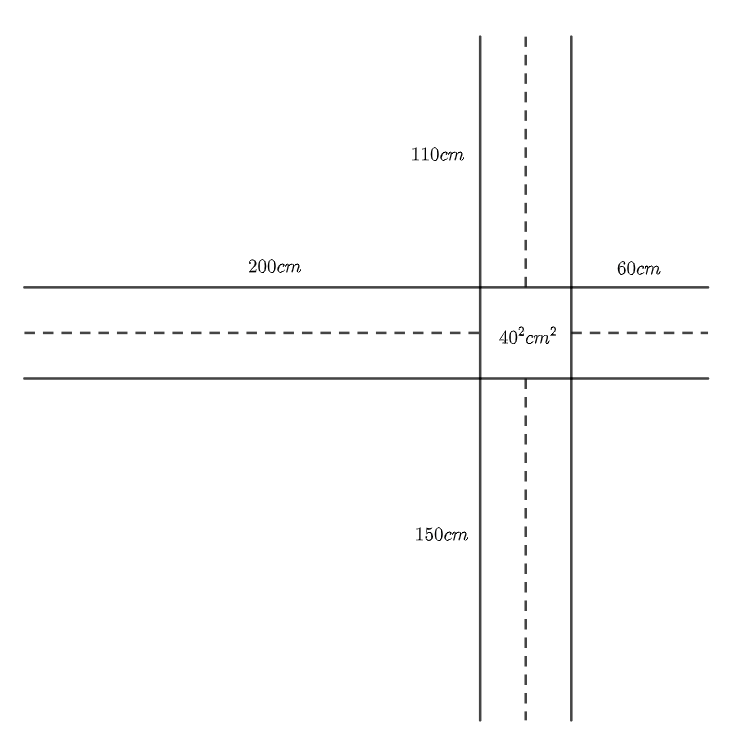
\includegraphics[width=1\linewidth]{figures/alt_intersection_config}
	\caption{An alternative configuration of the intersection and its connected roads by adding extra parameter to the initialization of the intersection as described by the previous code snippet.}
	\label{fig:altintersectionconfig}
\end{figure}

The length is in centimeters and needs to correlate with the length of the physical track. We used tape to show where the roads were. However, this is unnecessary. We recommend a track between three to four meters long for the best results.

Lastly, position both vehicles down at the start of the two tracks, turn on the server and connect to the power banks. The vehicles should automatically connect to the server after 20-30 seconds. When both vehicles have established a connection to the server, the demonstration has started.
% \section{Preface}

The product documentation is a technical description of the product.

The product documentation assumes the reader has some prior knowledge in basic programming.
% \section{Program description}

\begin{figure}[h!]
	\centering
	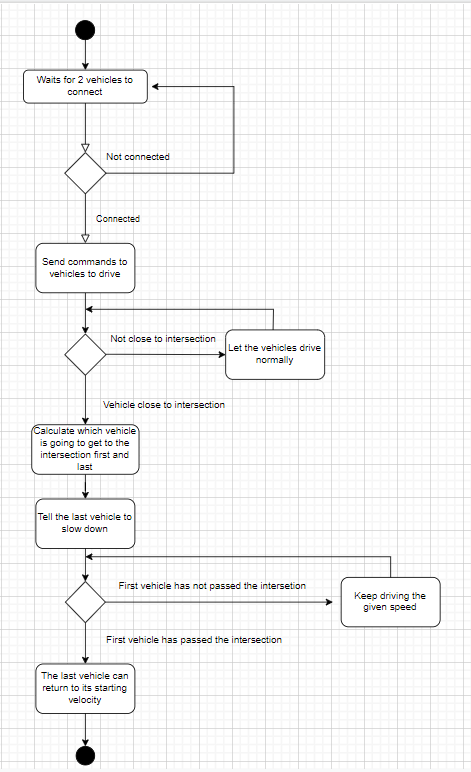
\includegraphics[width=1\linewidth]{figures/Flow_diagram_server}
	\caption[Flow diagram server]{Flow diagram for the server. This diagram specificly shows the flow of the semi physical demonstration.}
	\label{fig:diagramserver}
\end{figure}

The program is an IoT-system were vehicles can communicate with eachother through a server. It constists of a server which has the responsibility for the calculations and decision making, and a client which are the vehicles. The function of the program is to increase traffic flow and prevent traffic congestion. As of now the program can be used in an intersection with two vehicles, but can be scaled to include more vehicles. Here is a diagram that describes the flow of our server in the demonstration:




% \section{Adherence to project requirements}
Our solution adheres to the requirements Accenture set for us. Our prototype cars can work both with, and without being connected to a server. The server can handle multiple connections and adjust trafic based on the situation on the road. Through er deomnstration we also showed a situation where the outcome differs depending on if the cars are connected to the server or just driving on the on-board AI.


% \section{Server flow diagram}


